\section{Redes neuronales}

En 1943 ya exist\'ia una comunidad animada de biof\'isicos que realizaban trabajos matem\'aticos en redes neuronales. t\'erminos de lo que se conoci\'o como TuringMachines, para explicar c\'omo los mecanismos neuronales podr\'ian realizar funciones mentales.

Warren McCulloch y Walter Pitts (1943) crearon un modelo inform\'atico para redes neuronales, que se llama l\'ogica umbral, que se base en las matem\'aticas y los algoritmos. Este modelo se\~nal\'o el camino para que la investigaci\'on de redes neuronales se divida en dos enfoques distintos. Un enfoque se centr\'o en los procesos biol\'ogicos en el cerebro y el otro se centr\'o en la aplicaci\'on de redes neuronales para la inteligencia artificial.

Un avance clave posterior fue el algoritmo de propagaci\'on hacia atr\'as que resuelve eficazmente el problema de o-exclusivo, y en general el problema del entrenamiento r\'apido de redes neuronales de m\'ultiples capas (Werbos 1975). El proceso de propagaci\'on hacia atr\'as utiliza la diferencia entre el resultado producido y el resultado deseado para cambiar los <<pesos>> de las conexiones entre las neuronas artificiales.

\subsection{El mdelo biol\'ogico}
Desde que se empez\'o a conocer la anatom\'ia y estructura
del tejido nervioso,a partir de los trabajos de Ram\'on y
Cajal (1911) en Espa\~na, los investigadores trataron de
conocer la forma c\'omo este tejido y los \'organos que
constituye, especialmente el cerebro, procesan la
informaci\'on que reciben de los \'organos receptores, para dar
una respuesta adecuada a sus est\'imulos. Aunque aun se est\'a
lejos de comprender el funcionamiento y la estructura del
sistema nervioso, se conoce con cierto detalle la estructura
de la neurona, como elemento b\'asico del tejido nervioso y la
forma c\'omo se estructura la corteza cerebral.

La neurona, como toda c\'elula, consta de una membrana
exterior M, que la limita y le sirve de \'organo de
intercambio con el medio exterior, de un citoplasma C, que
es el cuerpo principal de la c\'elula donde radica el grueso
de sus funciones y de un n\'ucleo N, que contiene el material
gen\'etico de la c\'elula. 

\begin{figure}[H]
	\centering
	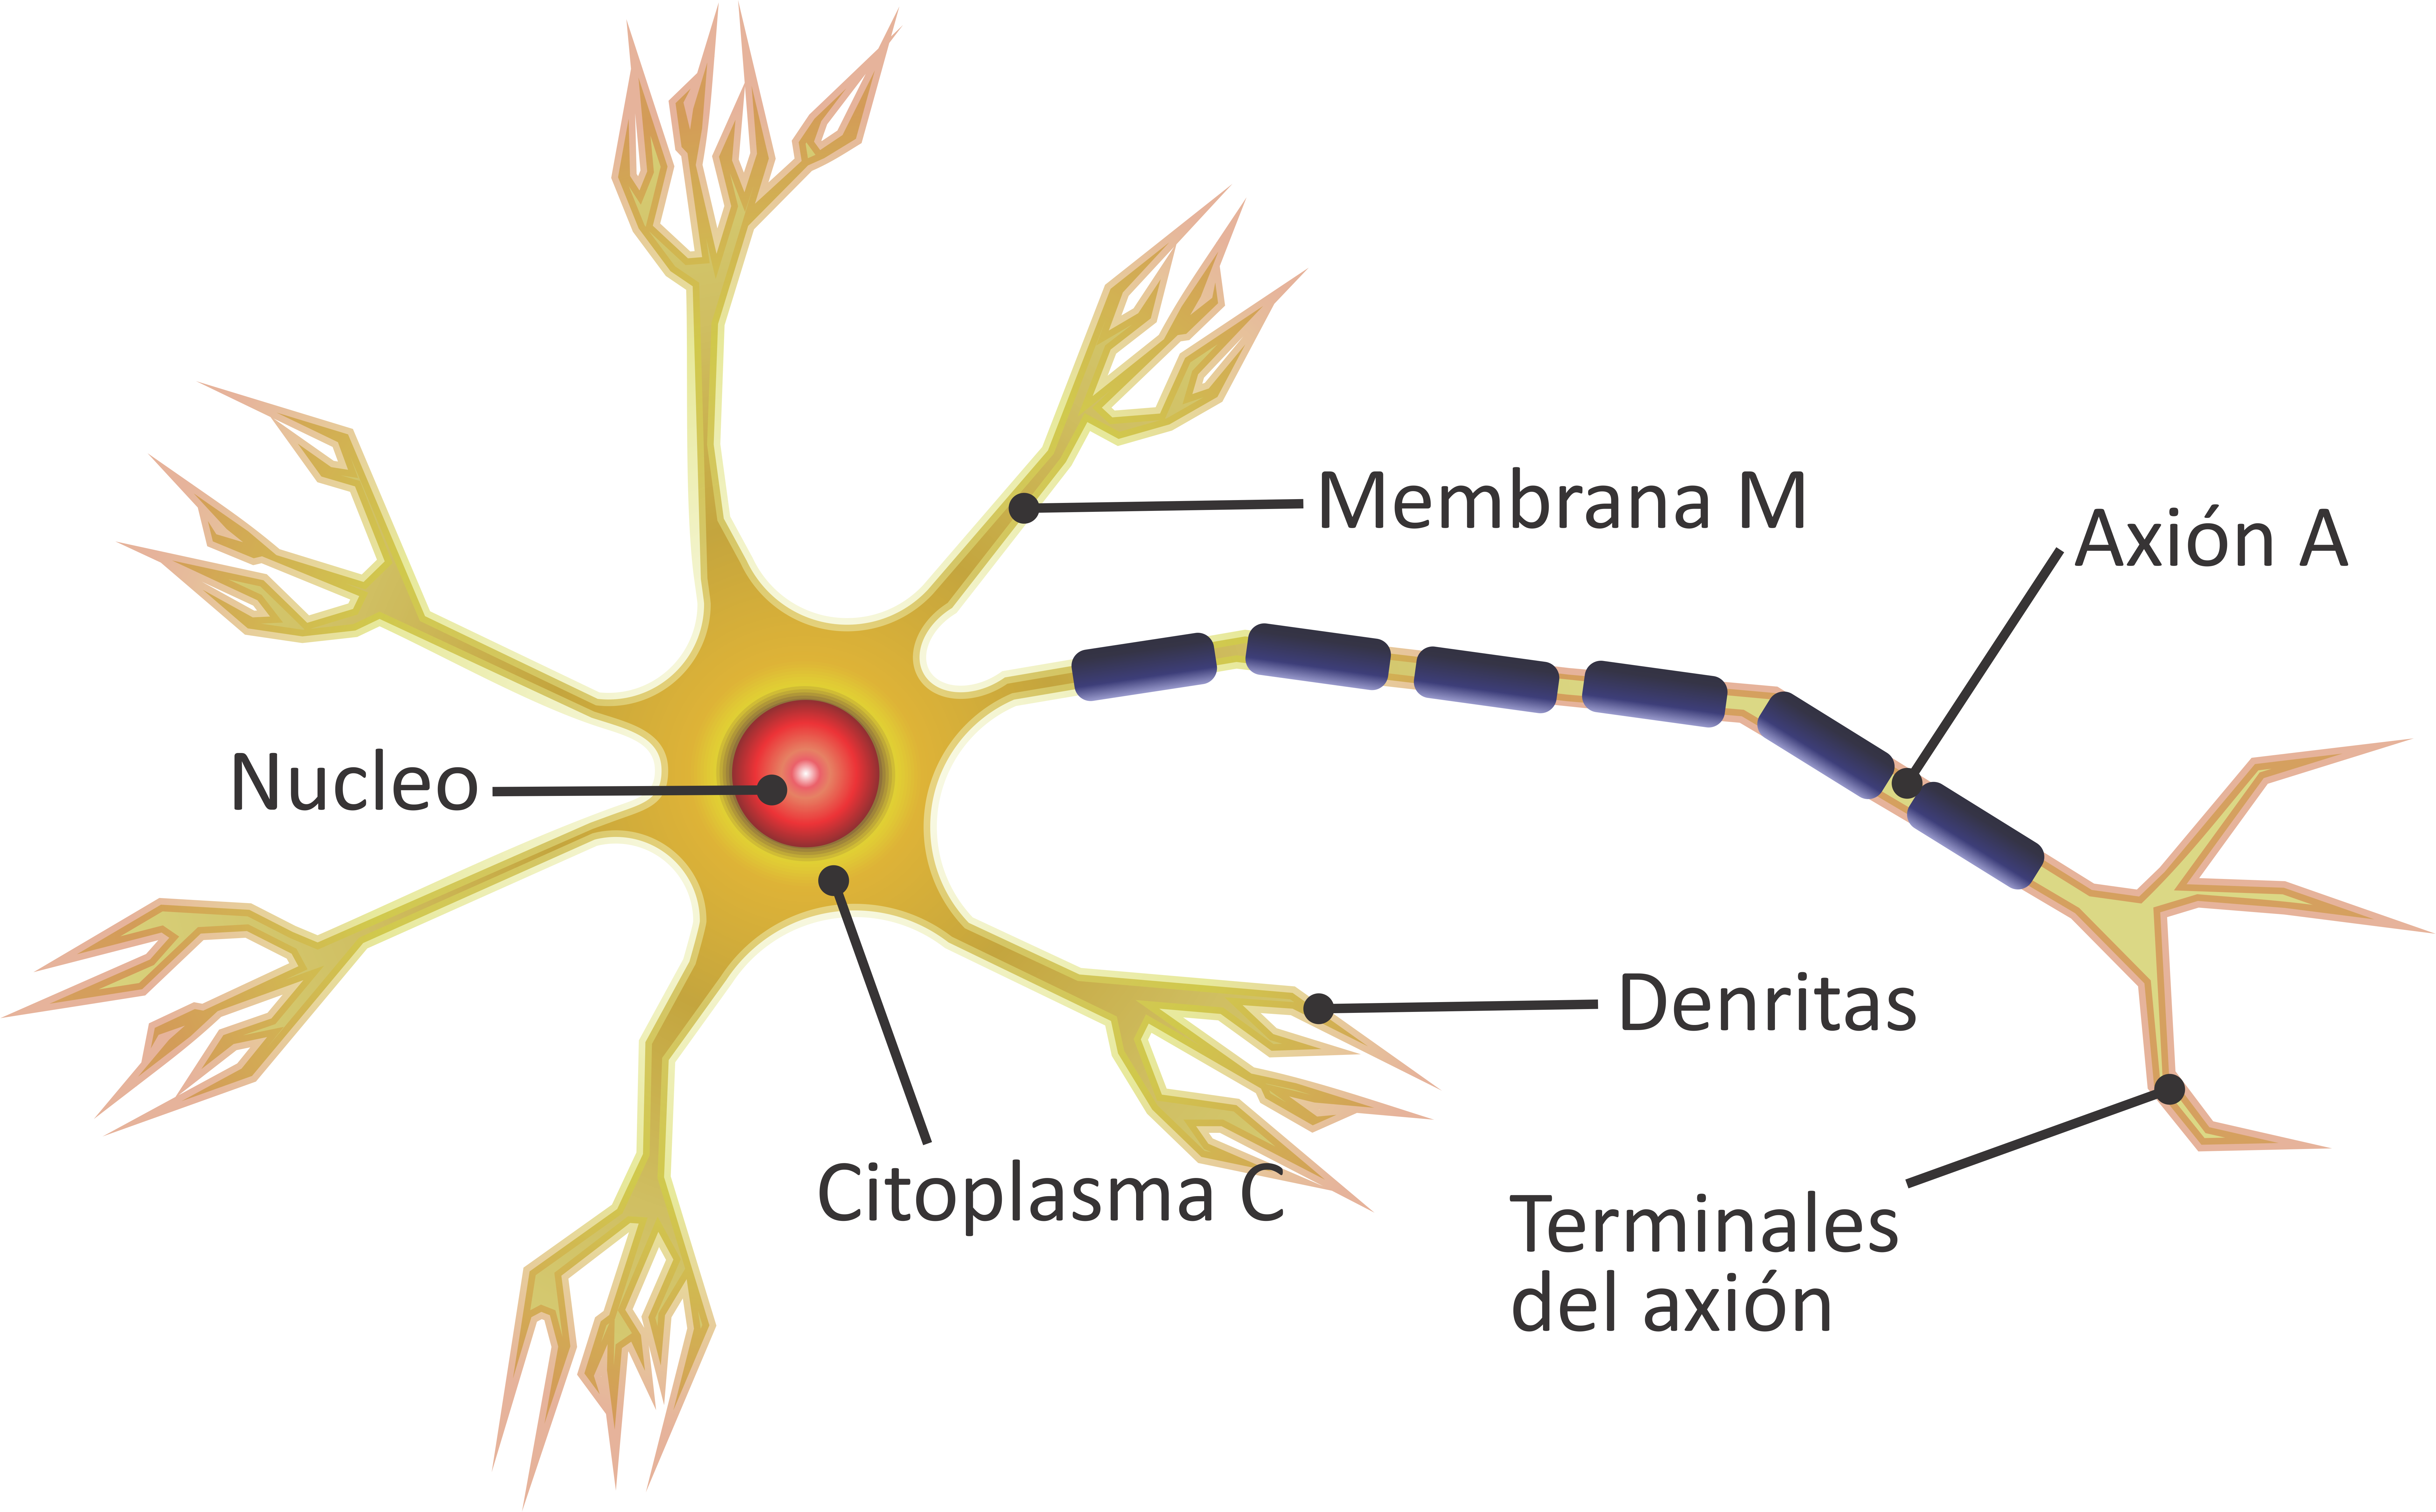
\includegraphics[width=7cm]{img/fig_neuronScheme.png}
	\caption{Esquema de una neurona.}
	\label{fig:neuronScheme}
\end{figure}

El citoplasma presenta unos alargamientos D, llamados 
dendritas, que son \'organos de recepci\'on. En las dendritas
termina un gran n\'umero de fibras F que son conductores que
llevan la se\~nal o impulso nervioso de los receptores o de
otras neuronas hacia la neurona. Estas fibras terminan en un
peque\~no corp\'usculo llamado sinapsis, que constituye un
relevador bioqu\'imico y que sirve para transferir la se\~nal de
una neurona a otra.

Existen dos clases de sinapsis: actuadoras, que
favorecen el disparo de la neurona receptora e inhibidoras,
que dificultan \'este. Cuando se presenta un cierto desbalance
entre las sinapsis actuadoras y las inhibidoras activas, la
neurona dispara un impulso de salida, que constituye la
respuesta de la neurona. Este impulso nervioso de salida es
conducido por una prolongaci\'on cil\'indrica alargada (hasta de
varios dec\'imetros de largo) de la neurona, que se llama
cilindro eje o ax\'on A, que en su extremo se divide en varias
fibras para comunicarse con otras neuronas o con \'organos
efectores o motores como gl\'andulas o m\'usculos.

El citoplasma de las neuronas forma la masa gris de los
centros nerviosos y el conjunto de cilindros ejes forma la
masa blanca de aqu\'ellos.
%http://conceptos.sociales.unam.mx/conceptos_final/598trabajo.pdf

\subsection{Modelo de neurona artificial}
La neurona artificial es una unidad procesadora con
cuatro elementos funcionales: 

\begin{figure}[H]
	\centering
	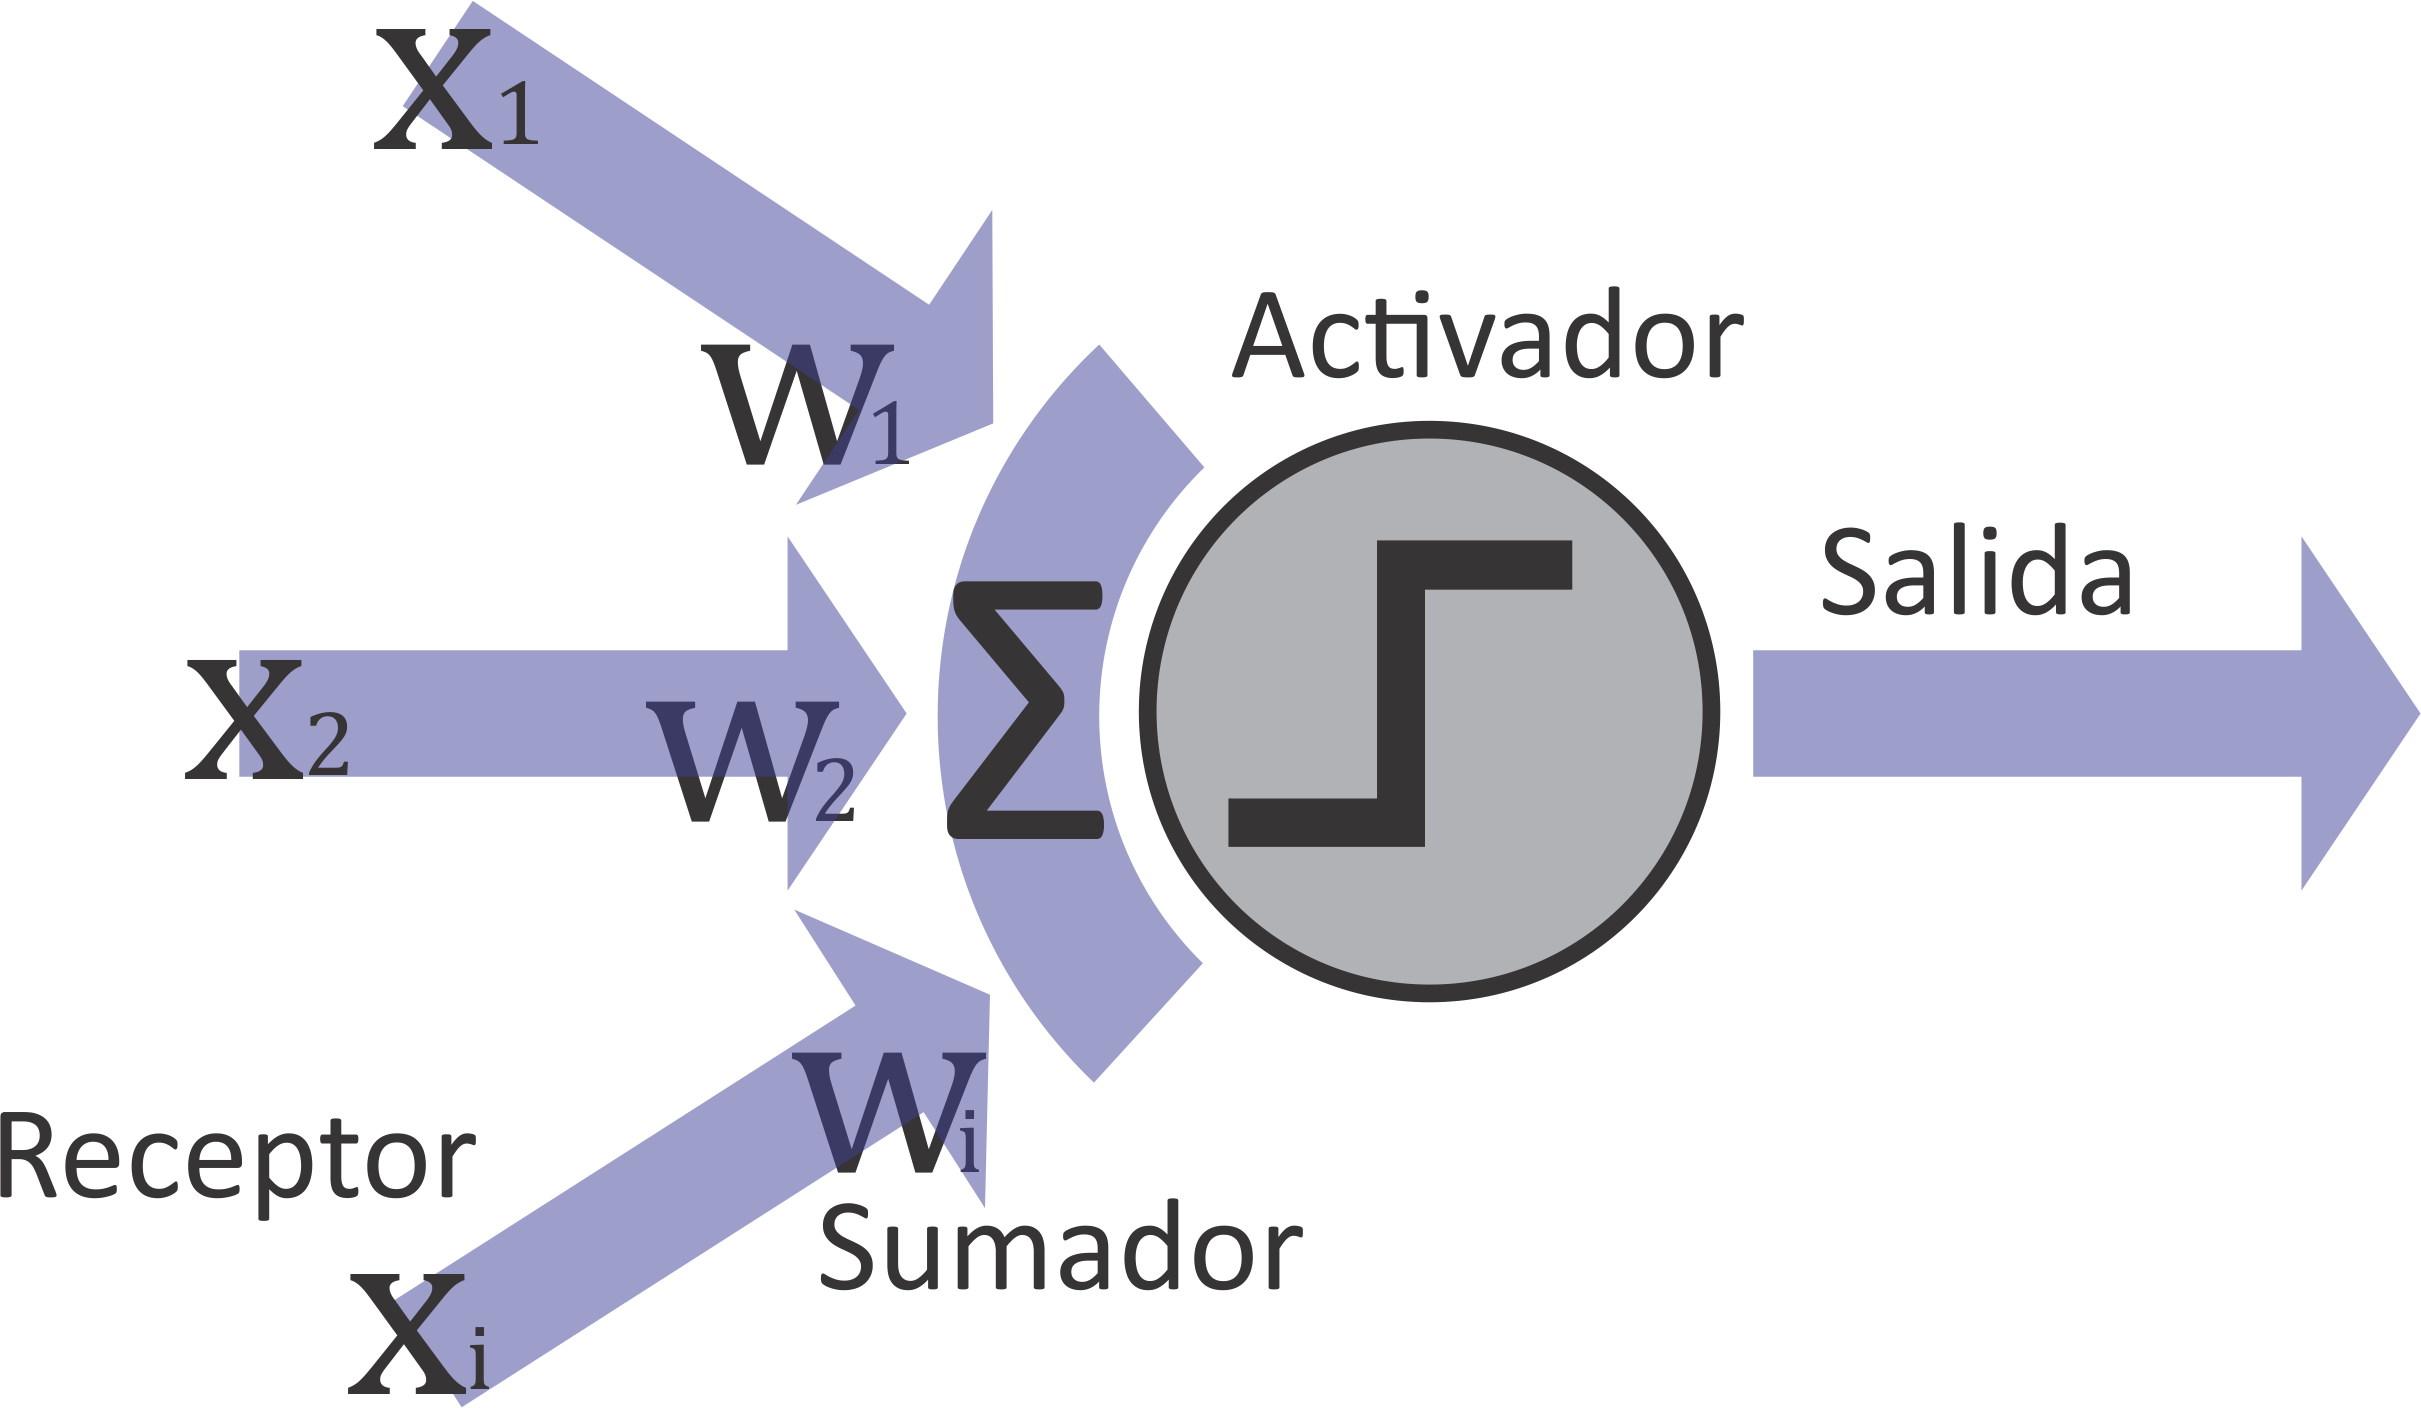
\includegraphics[width=5cm]{img/fig_artifitialNeuron.png}
	\caption{Esquema de una neurona.}
	\label{fig:artifitialNeuron}
\end{figure}

\begin{enumerate}
	\item El elemento receptor, a donde llegan una o varias
	se\~nales de entrada $x_i$, que generalmente provienen de otras
	neuronas y que son atenuadas o amplificadas cada una de
	ellas con arreglo a un factor de peso wi que constituye la
	conectividad entre la neurona fuente de donde provienen y la
	neurona de destino en cuesti\'on.

	\item El elemento sumador, que efect\'ua la suma algebraica
	ponderada de las se\~nales de entrada, ponder\'andolas de
	acuerdo con su peso, aplicando la siguiente expresi\'on: $s=\Sigma w_i x_i$

	\item El elemento de funci\'on activadora, que aplica una
	funci\'on no lineal de umbral (que frecuentemente es una
	funci\'on escal\'on o una curva log\'istica) a la salida del
	sumador para decidir si la neurona se activa, disparando una
	salida o no.

	\item El elemento de salida que es el que produce la se\~nal,
	de acuerdo con el elemento anterior, que constituye la
	salida de la neurona.
\end{enumerate}

Este modelo neuronal es el utilizado en casi todas las
Redes Neuronales artificiales, variando \'unicamente el tipo
de funci\'on activadora.

\subsubsection{Entradas y salidas}
Las entradas y salidas de una neurona pueden ser clasificadas en dos
grandes grupos, binarias o continuas. Las neuronas binarias (digitales) s\'olo
admiten dos valores posibles. En general en este tipo de neurona se utilizan los
siguientes dos alfabetos ${0,1}$ o ${-1,1}$. Por su parte, las neuronas continuas
(anal\'ogicas) admiten valores dentro de un determinado rango, que en general
suele definirse como $[-1, 1]$.
La selecci\'on del tipo de neurona a utilizar depende de la aplicaci\'on y del
modelo a construir.

\subsubsection{Pesos sin\'apticos}
El peso sin\'aptico wij define la fuerza de una conexi\'on sin\'aptica entre dos
neuronas, la neurona presin\'aptica i y la neurona postsin\'aptica j. Los pesos
sin\'apticos pueden tomar valores positivos, negativos o cero. En caso de una
entrada positiva, un peso positivo act\'ua como excitador, mientras que un peso
negativo act\'ua como inhibidor. En caso de que el peso sea cero, no existe
comunicaci\'on entre el par de neuronas.
Mediante el ajuste de los pesos sin\'apticos la red es capaz de adaptarse a
cualquier entorno y realizar una determinada tarea.

\subsubsection{Funci\'on de activaci\'on}
La funci\'on de activaci\'on determina el estado de activaci\'on actual de la
neurona

La tabla \ref{table:activationFunctions} muestra un listado de algunas de las funciones de activaci\'on
m\'as utilizadas en los distintos modelos de redes neuronales artificiales. 
\begin{table}[ht]
	\caption{}
	\label{table:activationFunctions}
	\begin{center}
		\begin{tabular}{ |c|c|c| }
			\hline
			Nombre & Funci\'on & Rango \\
			\hline
			Identidad &
			$x=y$ &
			$[-\infty,\infty]$ \\
			\hline
			Escal\'on &
			\begin{tabular}{ c }
				$y=1 $si$ x\geq 0$ \\
				$y=0 $si$ x<0$ \\
				\hline
				\hline
				$y=1 $si$ x\geq 0$ \\
				$y=-1 $si$ x<0$ \\
			\end{tabular} &
			\begin{tabular}{ c }
				$[0,1]$ \\
				\hline
				\hline
				$[-1,1]$
			\end{tabular} \\
			\hline
			Lineal a tramos &
			\begin{tabular}{ c }
				$y=x $si$ -1<x<1$ \\
				$y=1 $si$ x>1$ \\
				$y=-1 $si$ x<-1$ \\
			\end{tabular} &
			$[-1,1]$ \\
			\hline
			Sigmoide &
			$y=\frac{1}{1+\exp^-x}$ &
			$[0,1]$ \\
			\hline
			Sinusoidal &
			$y=sen(wx+\Phi)$ &
			$[-1,1]$ \\
			\hline
		\end{tabular}
	\end{center}
\end{table}
%http://conceptos.sociales.unam.mx/conceptos_final/598trabajo.pdf
%http://laboratorios.fi.uba.ar/lsi/bertona-tesisingenieriainformatica.pdf

\subsection{Arquitectura de una red neuronal}
Una vez definida el tipo de neurona que se utilizar\'a en un modelo de redes
neuronales artificiales es necesario definir la topolog\'ia de la misma.
La organizaci\'on y disposici\'on de las neuronas dentro de una red neuronal
se denomina topolog\'ia, y viene dada por el n\'umero de capas, la cantidad de
neuronas por capa, el grado de conectividad, y el tipo de conexi\'on entre
neuronas.
Las neuronas suelen agruparse en unidades funcionales denominadas
capas. Se denomina capa de entrada a aquella que esta compuesta por
neuronas de entradas y por lo tanto recibe informaci\'on procedente desde el
exterior. An\'alogamente, se denomina capa oculta y capa de salida a aquellas
capas que est\'an compuestas por neuronas ocultas y de salida
respectivamente. Una red neuronal artificial esta compuesta por una o m\'as
capas, las cuales se encuentran interconectadas entre s\'i.
Entre un par de neuronas de la red neuronal artificial pueden existir
conexiones. Estas conexiones son las sinapsis, tienen asociadas un peso
sin\'aptico, y son direccionales.
Cuando la conexi\'on se establece entre dos neuronas de una misma capa
hablamos de conexiones laterales o conexiones intra-capa. Por el contrario, si
la conexi\'on se establece entre neuronas de distintas capas se la denomina
conexi\'on inter-capa. Si la conexi\'on se produce en el sentido inverso al de
entrada-salida la conexi\'on se llama recurrente o realimentada.
Una red puede estar formada por una \'unica capa de neuronas. En este
caso hablamos de redes monocapa, y las neuronas que conforman dicha capa
cumplen la funci\'on de neuronas de entrada y salida simult\'aneamente. Cuando
la red esta compuesta por dos o m\'as capas hablamos de redes multicapa.
A su vez, hablamos de redes neuronales con conexi\'on hacia delante (redes
feedforward) cuando las conexiones entre las distintas neuronas de la red
siguen un \'unico sentido, desde la entrada de la red hacia la salida de la misma.
Cuando las conexiones pueden ser tanto hacia delante como hacia atr\'as
hablamos de redes recurrentes (redes feedback).
%http://laboratorios.fi.uba.ar/lsi/bertona-tesisingenieriainformatica.pdf

\subsection{Aprendizaje}
Durante la operatoria de una red neuronal podemos distinguir claramente
dos fases o modos de operaci\'on: la fase de aprendizaje o entrenamiento, y la
fase de operaci\'on o ejecuci\'on.
Durante la primera fase, la fase de aprendizaje, la red es entrenada para
realizar un determinado tipo de procesamiento. Una vez alcanzado un nivel de
entrenamiento adecuado, se pasa a la fase de operaci\'on, donde la red es
utilizada para llevar a cabo la tarea para la cual fue entrenada.

\subsubsection{Fase de entrenamiento}
Una vez seleccionada el tipo de neurona artificial que se utilizar\'a en una red
neuronal y determinada su topolog\'ia es necesario entrenarla para que la red
pueda ser utilizada. Partiendo de un conjunto de pesos sin\'apticos aleatorio, el
proceso de aprendizaje busca un conjunto de pesos que permitan a la red
desarrollar correctamente una determinada tarea. Durante el proceso de
aprendizaje se va refinando iterativamente la soluci\'on hasta alcanzar un nivel
de operaci\'on suficientemente bueno.

El proceso de aprendizaje se puede dividir en tres grandes grupos de
acuerdo a sus caracter\'isticas

\begin{itemize}
	\item Aprendizaje supervisado. Se presenta a la red un conjunto de
	patrones de entrada junto con la salida esperada. Los pesos se van
	modificando de manera proporcional al error que se produce entre la
	salida real de la red y la salida esperada.
	\item Aprendizaje no supervisado. Se presenta ala red un conjunto de
	patrones de entrada. No hay informaci\'on disponible sobre la salida
	esperada. El proceso de entrenamiento en este caso deber\'a ajustar
	sus pesos en base a la correlaci\'on existente entre los datos de
	entrada.
	\item Aprendizaje por refuerzo. Este tipo de aprendizaje se ubica entre
	medio de los dos anteriores. Se le presenta a la red un conjunto de
	patrones de entrada y se le indica a la red si la salida obtenida es o
	no correcta. Sin embargo, no se le proporciona el valor de la salida
	esperada. Este tipo de aprendizaje es muy \'util en aquellos casos en
	que se desconoce cual es la salida exacta que debe proporcionar la
	red. 
\end{itemize}

\subsubsection{Fase de operaci\'on}
Una vez finalizada la fase de aprendizaje, la red puede ser utilizada para
realizar la tarea para la que fue entrenada. Una de las principales ventajas que
posee este modelo es que la red aprende la relaci\'on existente entre los datos,
adquiriendo la capacidad de generalizar conceptos. De esta manera, una red
neuronal puede tratar con informaci\'on que no le fue presentada durante de la
fase de entrenamiento.
%http://laboratorios.fi.uba.ar/lsi/bertona-tesisingenieriainformatica.pdf

